\documentclass[]{article}
\usepackage{geometry}
\geometry{
a4paper,
total={170mm,257mm},
left=20mm,
top=20mm,
}
\usepackage{graphicx}
\usepackage{subcaption}
\usepackage{listings}
\usepackage[justification=centering]{caption}
\usepackage{hyperref}
\usepackage{enumitem}
\usepackage[utf8]{inputenc}
\usepackage{float}
\DeclareTextFontCommand{\helvetica}{\fontfamily{phv}\selectfont}
\setlength{\parindent}{4em}
\setlength{\parskip}{1em}
\linespread{1.5}

\usepackage[table]{xcolor}
\usepackage{graphicx}
\usepackage{adjustbox}

\title{PAC2 Desenvolupament del treball - Fase 1}
\date{15 d'Abril 2019}
\author{Vasyl Druchkiv \\ Estudiant del Màster de Bioestadística i Bioinformàtica}
\renewcommand{\contentsname}{Índice}
\usepackage{setspace}


\renewcommand\paragraph{\@startsection{paragraph}{4}{\z@}%
{-2.5ex\@plus -1ex \@minus -.25ex}%
{1.25ex \@plus .25ex}%
{\normalfont\normalsize\bfseries}}

\begin{document}
\maketitle
\makeatletter

\makeatother
\begin{spacing}{0.1}
\tableofcontents
\end{spacing}



\section{Descripció de l'avenç del projecte} 

A data d'avui he desenvolpupat l'aplicació d'anàlisis de les rutes. L'aplicació és completament funcional localment i ofereix l'anàlisi a partir de les bases de dedes GO, KEGG i Reactome. A l'apartat \textbf{Input data} l'usuari primer ha d'indicar l'espècie per a totes tres bases de dades. Per les bases de dades GO i Reactome l'usuari pot elegir entre "human", "rat", "mouse", "celegans", "yeast", "zebrafish", "fly". Hi ha més espècies disponobles per a l'anàlisis KEGG, perquè la funció de \helvetica{culsterProfiler} \helvetica{enrichKEGG()} descarrega les últimes anotacions directament de la base de dades KEGG. Es poden trobar totes les espècies \href{http://www.genome.jp/kegg/catalog/org_list.html}{aquí}. També l'usuari pot buscar l'espècie introduint els termes de cerca. Finalment l'usuari puja l'arxiu amb els gens i els LogRatios provinents de l'estudi de microarrays o NGS. 

\begin{figure}[h!]
\caption{Pàgina d'entrada}
\centering
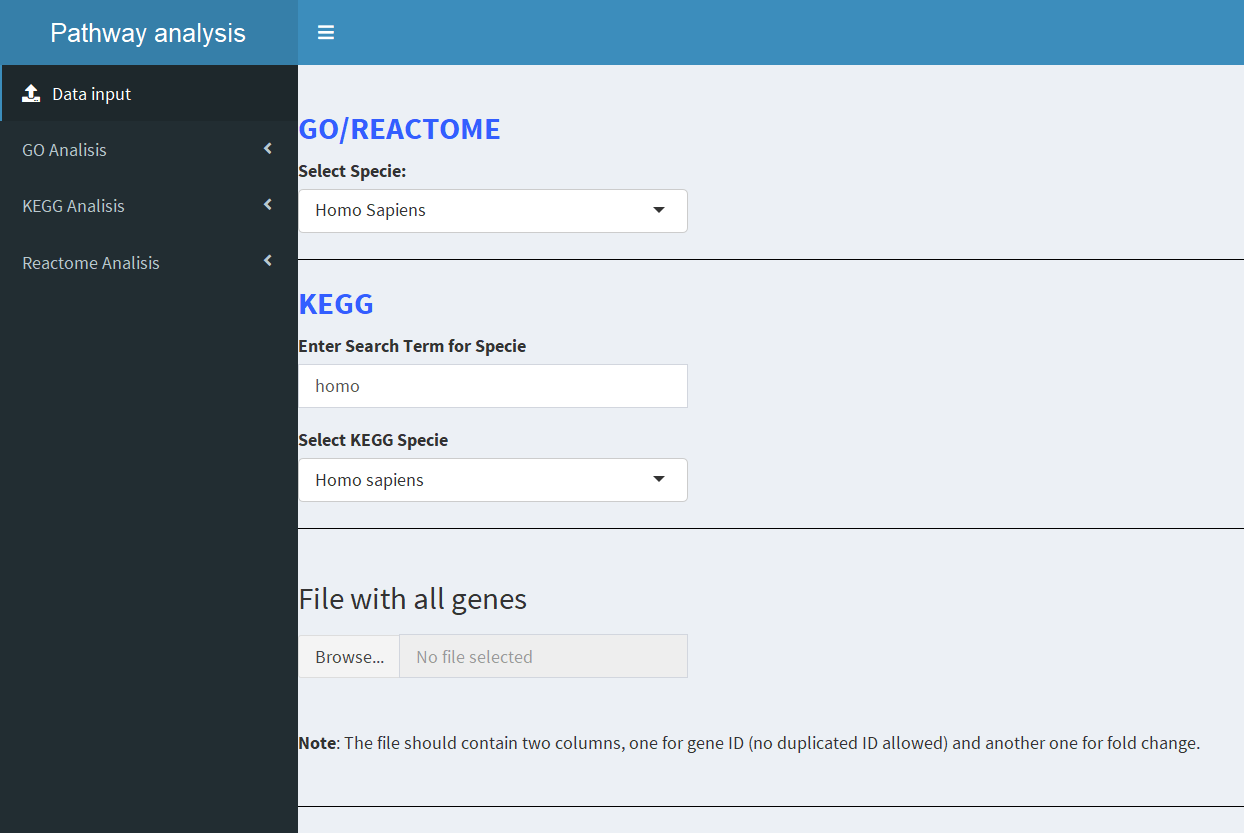
\includegraphics[width=0.9\textwidth]{App_F1}
\end{figure}

Un cop introduïdes les dades es mostra  un petit resum del contingut i es dona la possibilitat d'elegir el \textit{cut-off} de FoldChange per a l'anàlisi ORA. Per defecte s'agafa el valor de FoldChange=2. En funció del \textit{cut-off} elegit es mostra el nombre dels gens en aquest grup (gens sobre o sotaexpressats).

\begin{figure}[h!]
\caption{El resum de les dades selecció del \textit{cut off} per a l'anàlisi ORA}
\centering
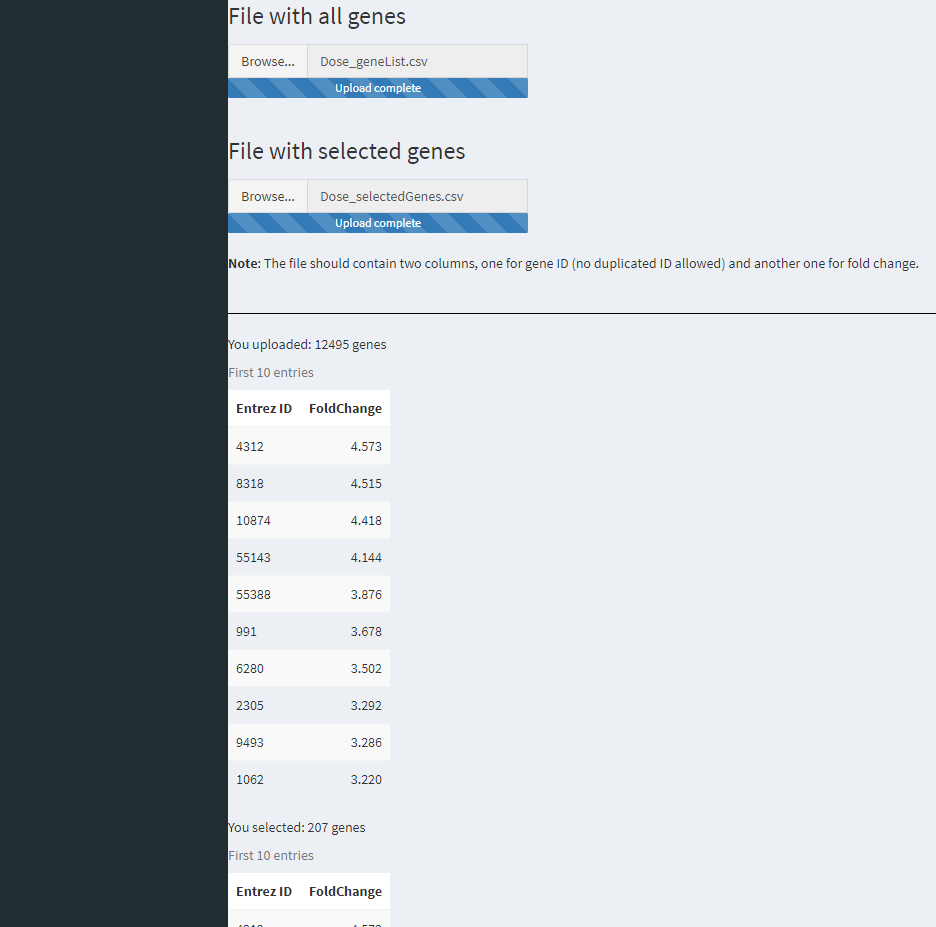
\includegraphics[width=0.9\textwidth]{App_F1b}
\end{figure}


L'aplicació està dividida doncs en 4 parts substancials:

\begin{enumerate}
\item Entrada de les dades;
\item Anàlisi GO;
\item Anàlisi KEGG;
\item Anàlisi Reactome.
\end{enumerate}


L'aplicació ofereix dos mètodes d'anàlisi: d'una banda es pot fer ORA (Over-Representation Analysis) i d'altra banda l'anàlisi GSEA (Gene Set Enrichment Analisis). Recordem que l'ORA consisteix a seleccionar els gens diferencialment expressats i basant-se en GO, KEGG o Reactome comprovar si una de les agrupacions de gens suggerides per aquestes bases de dades està sobre o sotraexpressada en els gens seleccionats. Per dur a terme l'ORA l'usuari té l’opció de definir un \textit{cut-off} de Log-Ratio per formar el conjunt dels gens que s'hi utilitzarà (\textit{gene set}). ORA és una bona eina per veure els efectes grans però els efectes petits se li escapen. Els efectes petits derivats dels gens individuals poden acumular-se en un efecte conjunt substancial el qual ORA no serà capaç de detectar. És aquí on GSEA mostra la seva utilitat. 

Els apartats d'anàlisi (GO, KEGG i Reactome) ofereixen tan representacions comunes com representacions específiques. 

Els anàlisis i representacions \underline{en comú} són:

\begin{itemize}
\item Taula dels resultats ORA;
\item Taula dels resultats GSEA;
\item Gràfic de barres del resultat ORA;
\item Gràfic de punts del resultat ORA;
\item El mapa d'enriquement (Enrichment Map);
\item La xarxa dels gens en categories (Category-gene-network);
\item El gràfic de GSEA.
\end{itemize} 

Les anàlisis \underline{específics} són:

\begin{itemize}
\item GO $\rightarrow$ Gràfic GO 
\item KEGG $\rightarrow$ Rutes de la base de dades KEGG
\item Reactome $\rightarrow$ Rutes de la base de dades Reactome
\end{itemize}

\begin{figure}[h!]
\centering
\begin{tabular}{ccc}
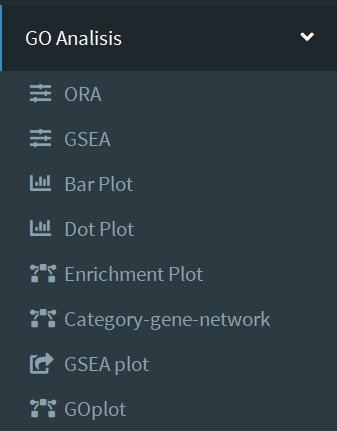
\includegraphics[width=45mm]{App_F2_Items_GO.png} & 
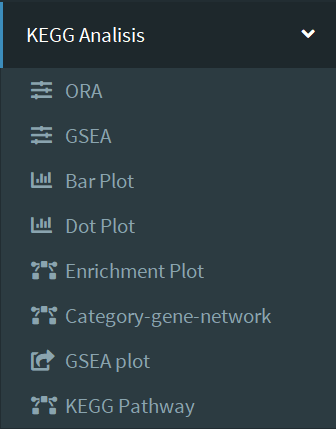
\includegraphics[width=45mm]{App_F3_Items_KEGG.png} &
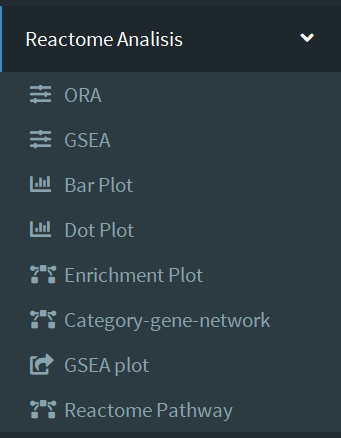
\includegraphics[width=45mm]{App_F4_Items_RA.png} \\
(a) GO & (b) KEGG & (c) Reactome \\
\end{tabular}
\caption{Els elements de les seccions d'anàlisi}
\end{figure}


\begin{table}[ht]
\begin{adjustbox}{width=1\textwidth}
\small
 \begin{tabular}{|| c | c | l | c | c ||} 
 \hline
 Base de dades & Mètode & Paquet Bioconductor & Funció & Observació \\ [0.5ex] 
 \hline\hline
 GO & ORA & clusterProfiler & enrichGO() & Només 7 espècies disponibles \\ 
 \hline
 GO & GSEA & clusterProfiler & gseGO() & Permutació de gens \\
 \hline
 GO & Bar-Plot & enrichplot & barplot() & Nececita l'objecte del class enrichResult \\
 \hline
 GO & Enrichment Map & enrichplot & emapplot() & Nececita l'objecte del class enrichResult \\
 \hline
 GO & Gene-Concept Network & enrichplot & cnetplot() & Nececita l'objecte del class enrichResult \\
 \hline
 GO & GO directed acyclic graph & enrichplot & goplot() & Nececita l'objecte del class enrichResult \\
 \hline\hline
 KEGG & ORA & clusterProfiler & enrichKEGG() & Totes les espècies de KEGG \\ 
 \hline
 KEGG & GSEA & clusterProfiler & gseKEGG() & Permutació de gens \\
 \hline
 KEGG & Bar-Plot & enrichplot & barplot() & Nececita l'objecte del class enrichResult \\
 \hline
 KEGG & Enrichment Map & enrichplot & emapplot() & Nececita l'objecte del class enrichResult \\
 \hline
 KEGG & Gene-Concept Network & enrichplot & cnetplot() & Nececita l'objecte del class enrichResult \\
 \hline
 KEGG & Pathway & pathview & pathview() & Cal modificar la funció per guardar els gràfics en el directori temporal \\
 \hline\hline
 Reactome & ORA & ReactomePA & enrichPathway() & Totes les espècies de KEGG \\ 
 \hline
 Reactome & GSEA & ReactomePA & gsePathway() & Permutació de gens \\
 \hline
 Reactome & Bar-Plot & enrichplot & barplot() & Nececita l'objecte del class enrichResult \\
 \hline
 Reactome & Enrichment Map & enrichplot & emapplot() & Nececita l'objecte del class enrichResult \\
 \hline
 Reactome & Gene-Concept Network & enrichplot & cnetplot() & Nececita l'objecte del class enrichResult \\
 \hline
 Reactome & Pathway & ReactomePA & viewPathway() & Molt llent. Per aquest motiu no he afegit botó de descarga. \\
 \hline
 \hline
\end{tabular}
\end{adjustbox}
\caption{Resum de les anàlisis disponibles i recursos de Bioconductor R} 
\end{table}

\section{L'anàlisi comuna de GO, KEGG i Reactome}

\subsection{ORA}

\subsubsection{GO}

Per realitzar l'anàlisi ORA per a termes GO s'utilitza la funció \helvetica{enrichGO} del paquet \helvetica{clusterPrifiler}.
\begin{lstlisting}[language=R]
enrichGO(gene, OrgDb, keyType = "ENTREZID", ont = "MF", pvalueCutoff = 0.05, 
pAdjustMethod = "BH", universe, qvalueCutoff = 0.2, minGSSize = 10, maxGSSize = 500, 
readable = FALSE, pool = FALSE)
\end{lstlisting}

He implementat els valors per defecte amb la possibilitat per a usuari d'elegir entre:

\begin{itemize}
\item \underline{Ontologies GO} 
\begin{itemize}
\item Molecular function, Biological proces, Cellular Components;
\end{itemize}
\item \underline{Nivell de significació basant-se en els valors de P ajustats}
\begin{itemize}
\item 0.1, 0.05, 0.01, 0.001;
\end{itemize}
\item \underline{Mètode d'ajustament}
\begin{itemize}
\item Holm; Hochberg; Hommel; Bonferroni; BH; BY; FDR; None.
\end{itemize}
\end{itemize}

\begin{figure}[h!]
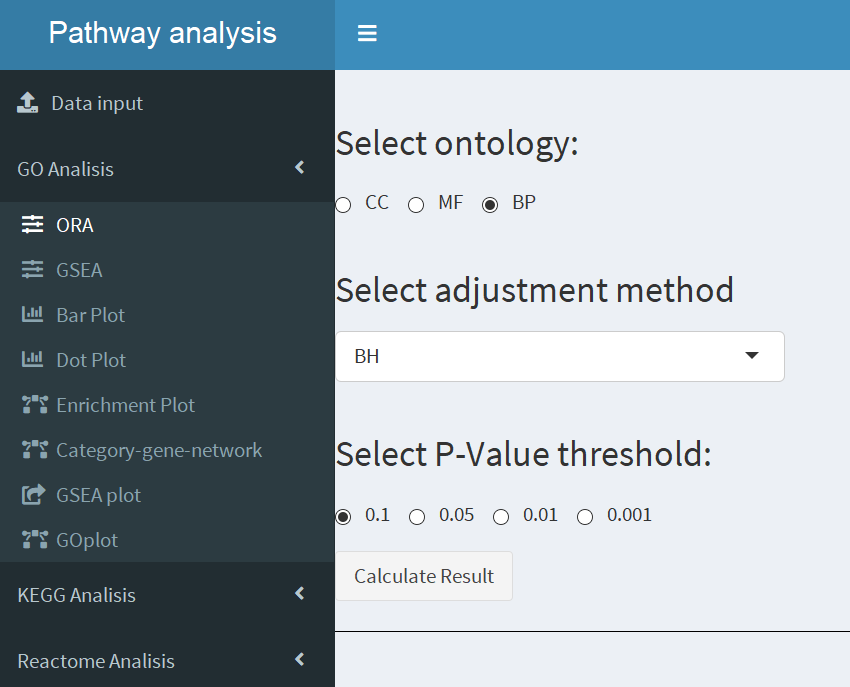
\includegraphics[width=0.9\textwidth]{App_F5_Items_GO_ORA.png}
\caption{Especificació d'ORA dels termes GO}
\end{figure}
L'execució de la funció és un procès temporalment costós. Per aquest motiu he afegit el botó d'acció, en lloc de deixar la funció reactiva. D'aquesta manera l'usuari ha de fer una decisió consient de repetir l'anàlisi amb altres valors.

Prement el botó apareix la taula i el botó nou mitjançant el qual l'usuari pot descarregar els resultats en format .csv. He formatejat la taula amb els paquets \helvetica{knitr}, \helvetica{kableExtra}, \helvetica{formattable} i \helvetica{dplyr}. Amb els dos últims he afegit les barres de color pel nombre dels gens diferencialment expressats del terme específic de GO i la gradacií de color del verd fins al vermell pels valors dels més petits fins els més grans. 

\begin{figure}[h!]
\centering
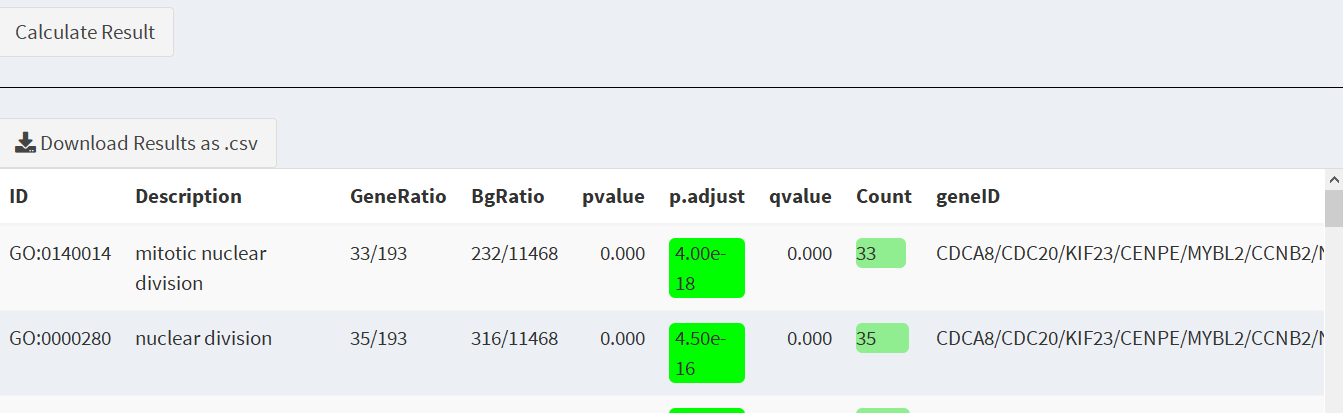
\includegraphics[width=0.9\textwidth]{App_F6_Items_GO_ORA_Table.png} 
\caption{El resultat d'anàlisi ORA. GO.}
\end{figure}

Els camps més interessants de la taula són:

\begin{itemize}
\item \underline{Description}. El nom del terme GO;
\item \underline{GeneRatio}. El quocient: $\displaystyle\frac{\mbox{Nombre dels gens diferencialment expressats que pertanyen al conjunt de gens}}{\mbox{Nombre total dels gens diferencialment expressats}}=\frac{M}{N}$; 
\item \underline{BgRatio}. El quocient: $\displaystyle\frac{\mbox{Nombre dels gens del conjunt d'interès en tota la mostra}}{\mbox{Nombre total dels gens  en la mostra}}=\frac{k}{n}$;
\item \underline{pvalue}. Valor de p basat en la distribució hipergeomètrica: $p = 1 - \displaystyle\sum_{i = 0}^{k-1}\frac{{M \choose i}{{N-M} \choose {n-i}}} {{N \choose n}}$
\item \underline{p.adjust}. El valor de P ajustat.
\end{itemize}

\subsubsection{KEGG}

Per l'ORA de base de dades KEGG he utilitzat la funció \helvetica{enrichKEGG()} del paquet \helvetica{clusterProfiler}. 

\begin{lstlisting}[language=R]
enrichKEGG(gene, organism = "hsa", keyType = "kegg", pvalueCutoff = 0.05, 
pAdjustMethod = "BH", universe, minGSSize = 10, maxGSSize = 500, 
qvalueCutoff = 0.2, use_internal_data = FALSE)
\end{lstlisting}



\begin{figure}[H]
\centering
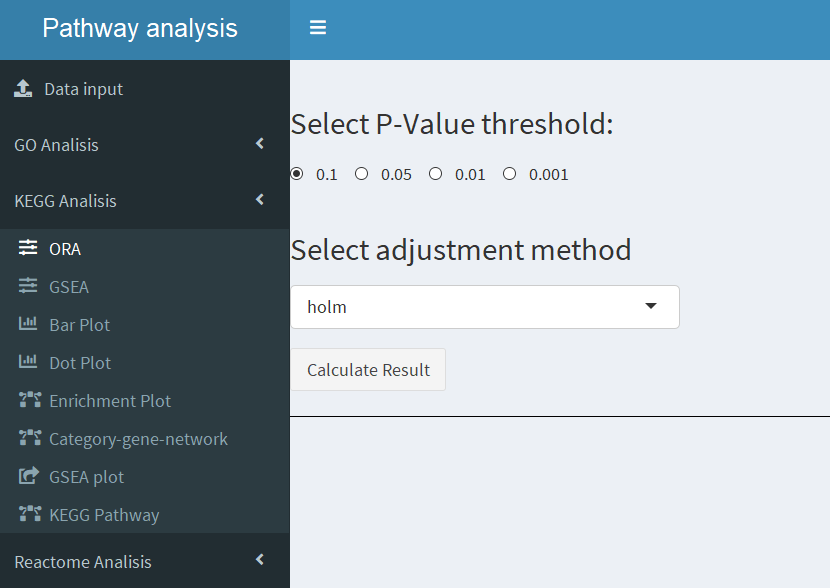
\includegraphics[width=0.9\textwidth]{App_F7_Items_KEGG_ORA.png} 
\caption{Configuració d'anàlisi KEGG}
\end{figure}



Una vegada introduïts els paràmetres i premut el botó \textbf{Calculate} apareix el botó \textbf{Download .csv} i la taula previsualitzada. Els camps de la taula són els mateixos com en l'anàlisi dels termes GO.
\begin{figure}[H]
\centering
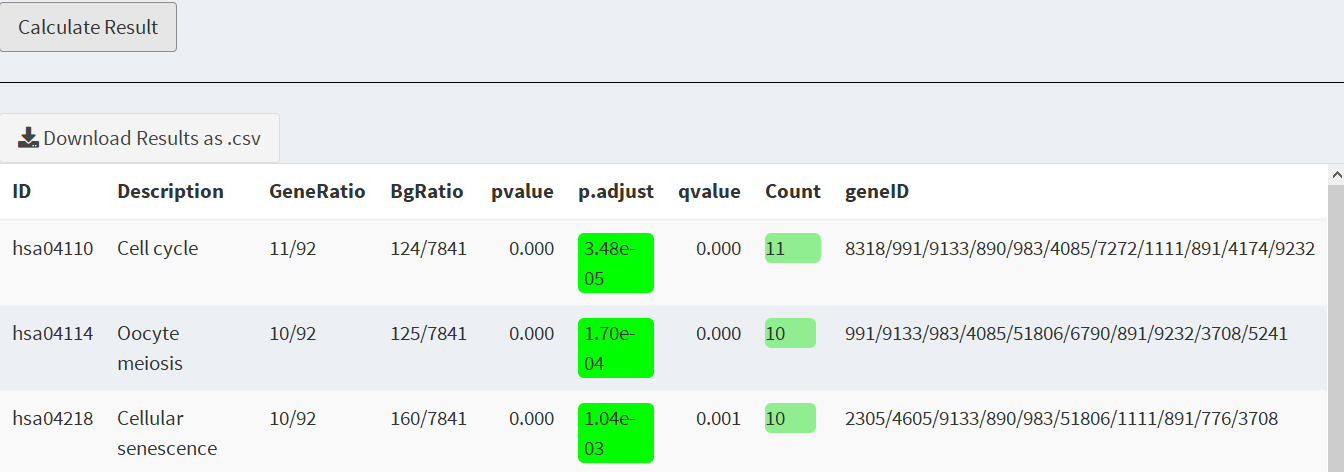
\includegraphics[width=0.9\textwidth]{App_F9_Items_KEGG_ORA_Table.png} 
\caption{El resultat de l'anàlisi ORA. KEGG.}
\end{figure}

\subsubsection{Reactome}
En el cas de Reactome el procediment és similar. La funció usada és \helvetica{enrichPathway()} del paquet \helvetica{ReactomePA}:

\begin{lstlisting}[language=R]
enrichPathway(gene, organism = "human", pvalueCutoff = 0.05,
pAdjustMethod = "BH", qvalueCutoff = 0.2, universe, minGSSize = 10,
maxGSSize = 500, readable = FALSE)
\end{lstlisting}


\begin{figure}[H]
\centering
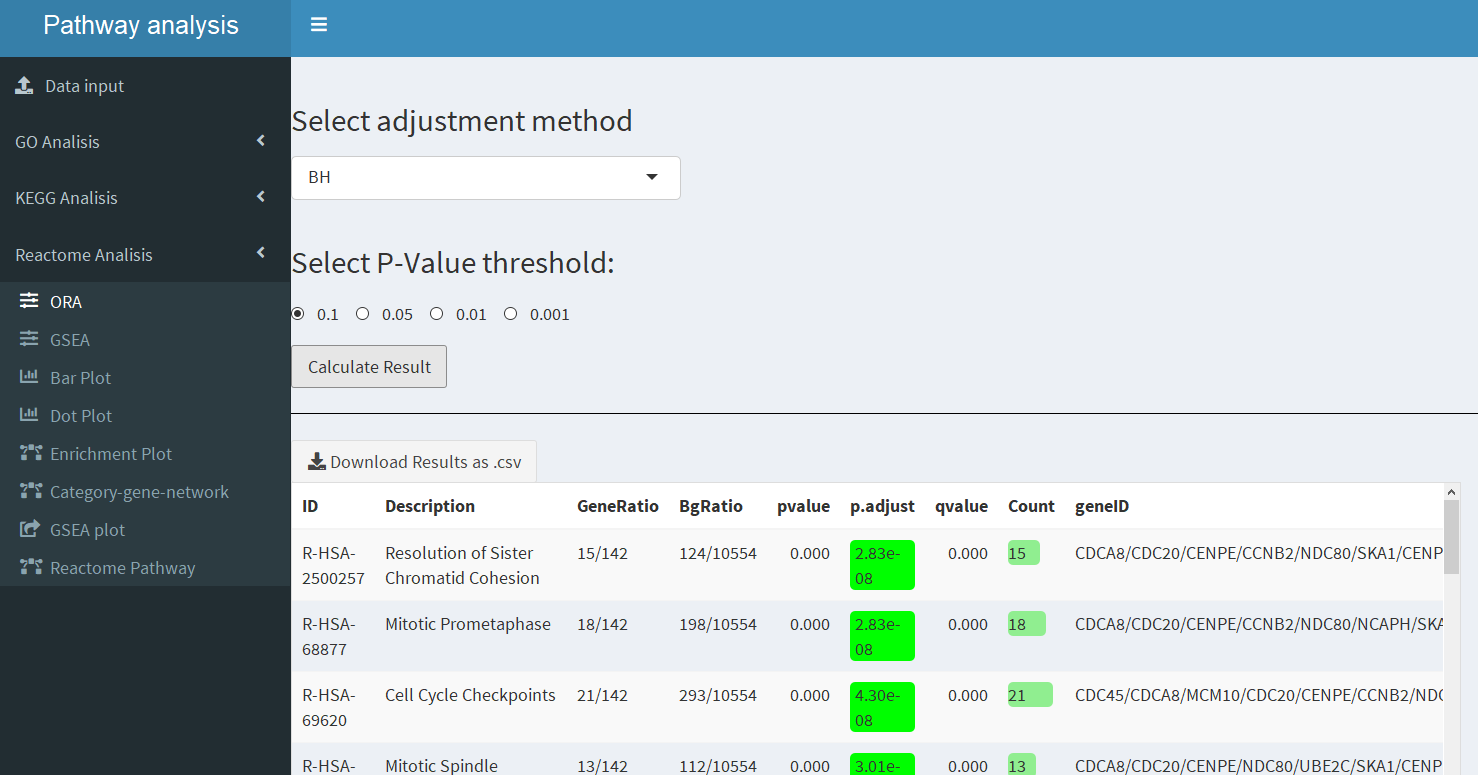
\includegraphics[width=0.9\textwidth]{App_F10_Items_Reactome_ORA.png} 
\caption{El resultat d'anàlisi ORA. Reactome.}
\end{figure}

\subsection{GSEA}
\subsubsection{GO}
El mètode GSEA per a termes GO es calcula amb la funció \helvetica{gseGO()} del paquet \helvetica{clusterProfiler}. 

\begin{lstlisting}[language=R]
gseGO(geneList, ont = "BP", OrgDb, keyType = "ENTREZID",
exponent = 1, nPerm = 1000, minGSSize = 10, maxGSSize = 500,
pvalueCutoff = 0.05, pAdjustMethod = "BH", verbose = TRUE,
seed = FALSE, by = "fgsea")
\end{lstlisting}

L'usuari pot elegir l'ontologia GO, el \textit{cut-off} del valor P i el mètode d'ajustament.
\begin{figure}[H]
\centering
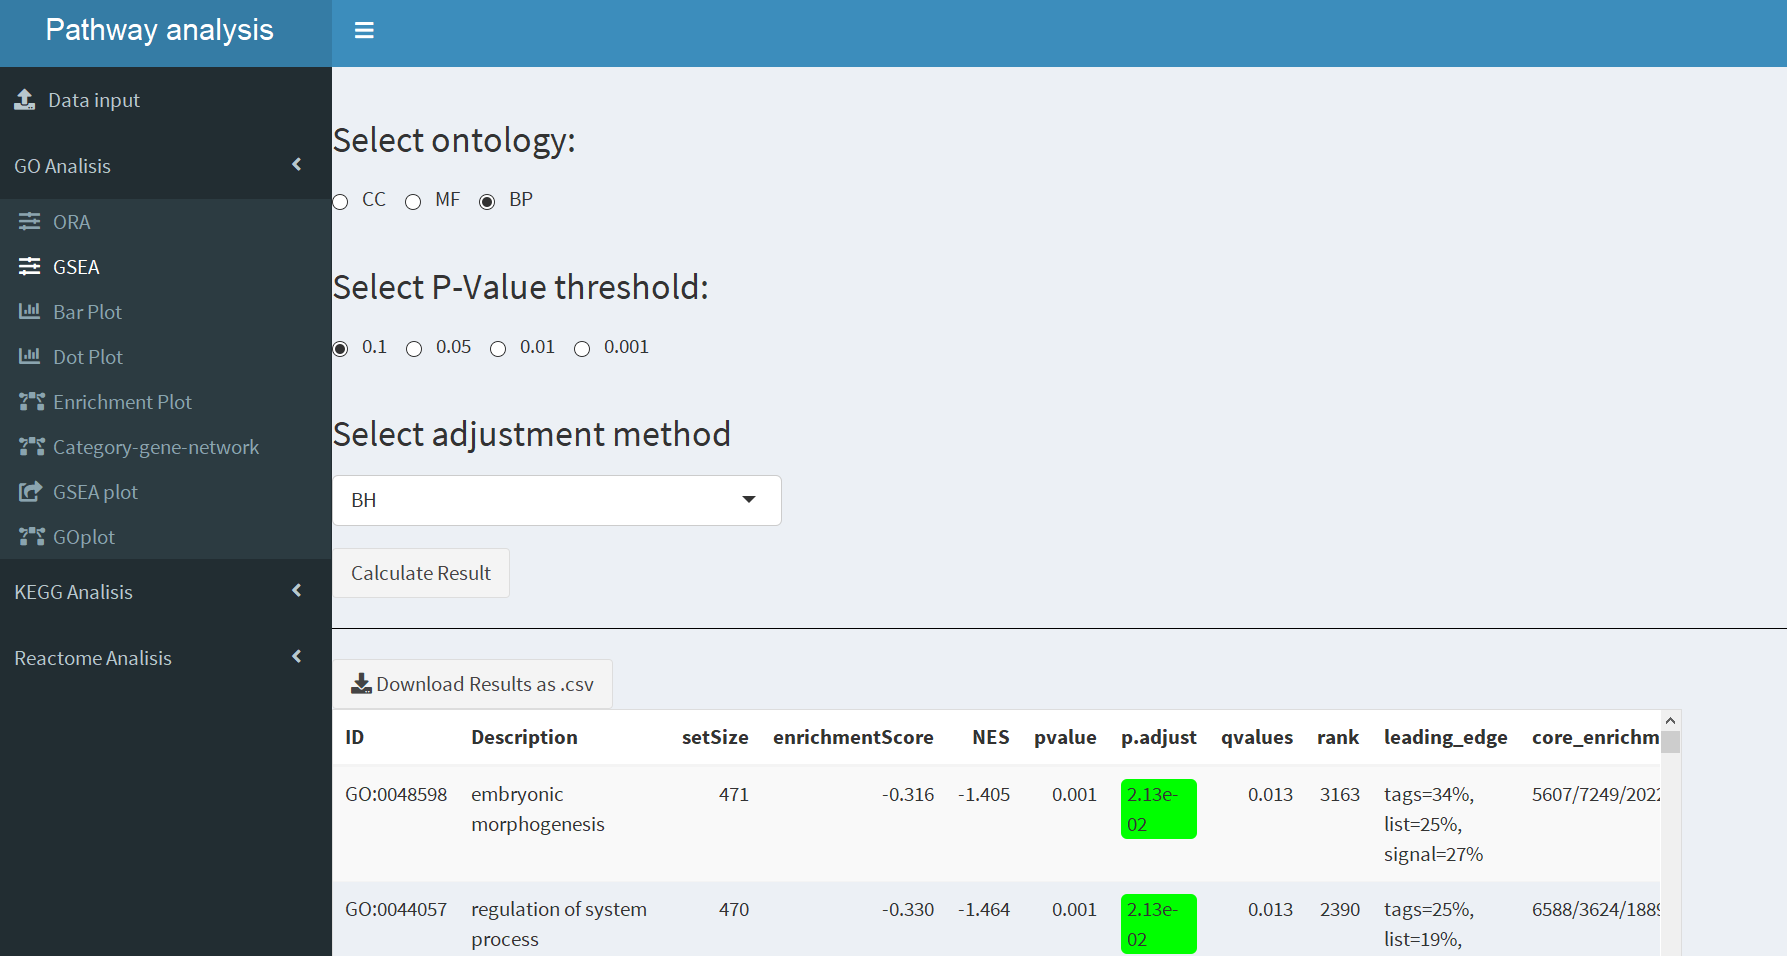
\includegraphics[width=0.9\textwidth]{App_F11_Items_GO_GSEA.png} 
\caption{El resultat de l'anàlisi GSEA. GO.}
\end{figure}

Per entendre l'anàlisi:



\begin{itemize}
\item \underline{enrichmentScore}. Enrichment score per al conjunt dels gens. Amb altres paraules: el grau amb el qual el conjunt dels gens està sobreexpressat a dalt o a baix del llistat ordenat dels gens en les dades d'expressió.
\item \underline{NES}. Normalized enrichment score. La puntuació per al conjunt de gens després de ser normalitzad tenint en compte tots els conjunts de gens analitzats (la seva mida i la seva correlació amb les dades d'expressió). Aquesta puntuació ajuda a comparar els resultats entre els conjunts de gens.
\item \underline{pvalue}.El valor de p nominal.
\item \underline{p.adjust}. El valor de p ajustat.
\item \underline{leading\_edge}
\begin{itemize}
\item \underline{Tags}. El percentatge de les ocurrències de gens del conjunt específic abans (per als ES positius) o després (per als ES negatius) del cim en la puntuació corrent d'enriquement. Aquest valor indica el percentatge dels gens que contribueixen a la puntuació d'enriquement. 
\item \underline{List}. El percentatge dels gens en el llistat ordenat de tots els gens abans o després del pic en la puntuació corrent d'enriquement. Aquest valor ens indica on exactament el pic es produeix. 
\item \underline{Signal}. La fortalesa del senyal d'enriquement que combina els dos valors anteriors.
\end{itemize}
\item \underline{rank}. La posició del pic en la llista ordenada dels gens. Els conjunts dels gens més interessants assoleixen el seu màxim o bé al principi o al final de la llista ordenada. Vol dir que tenen aquest valor o bé molt baix o bé molt alt.
\end{itemize}

\subsubsection{KEGG}
De la mateixa manera es calcula GSEA amb la funció \helvetica{gseKEGG()} del paquet \helvetica{clusterProfiler}:

\begin{figure}[H]
\centering
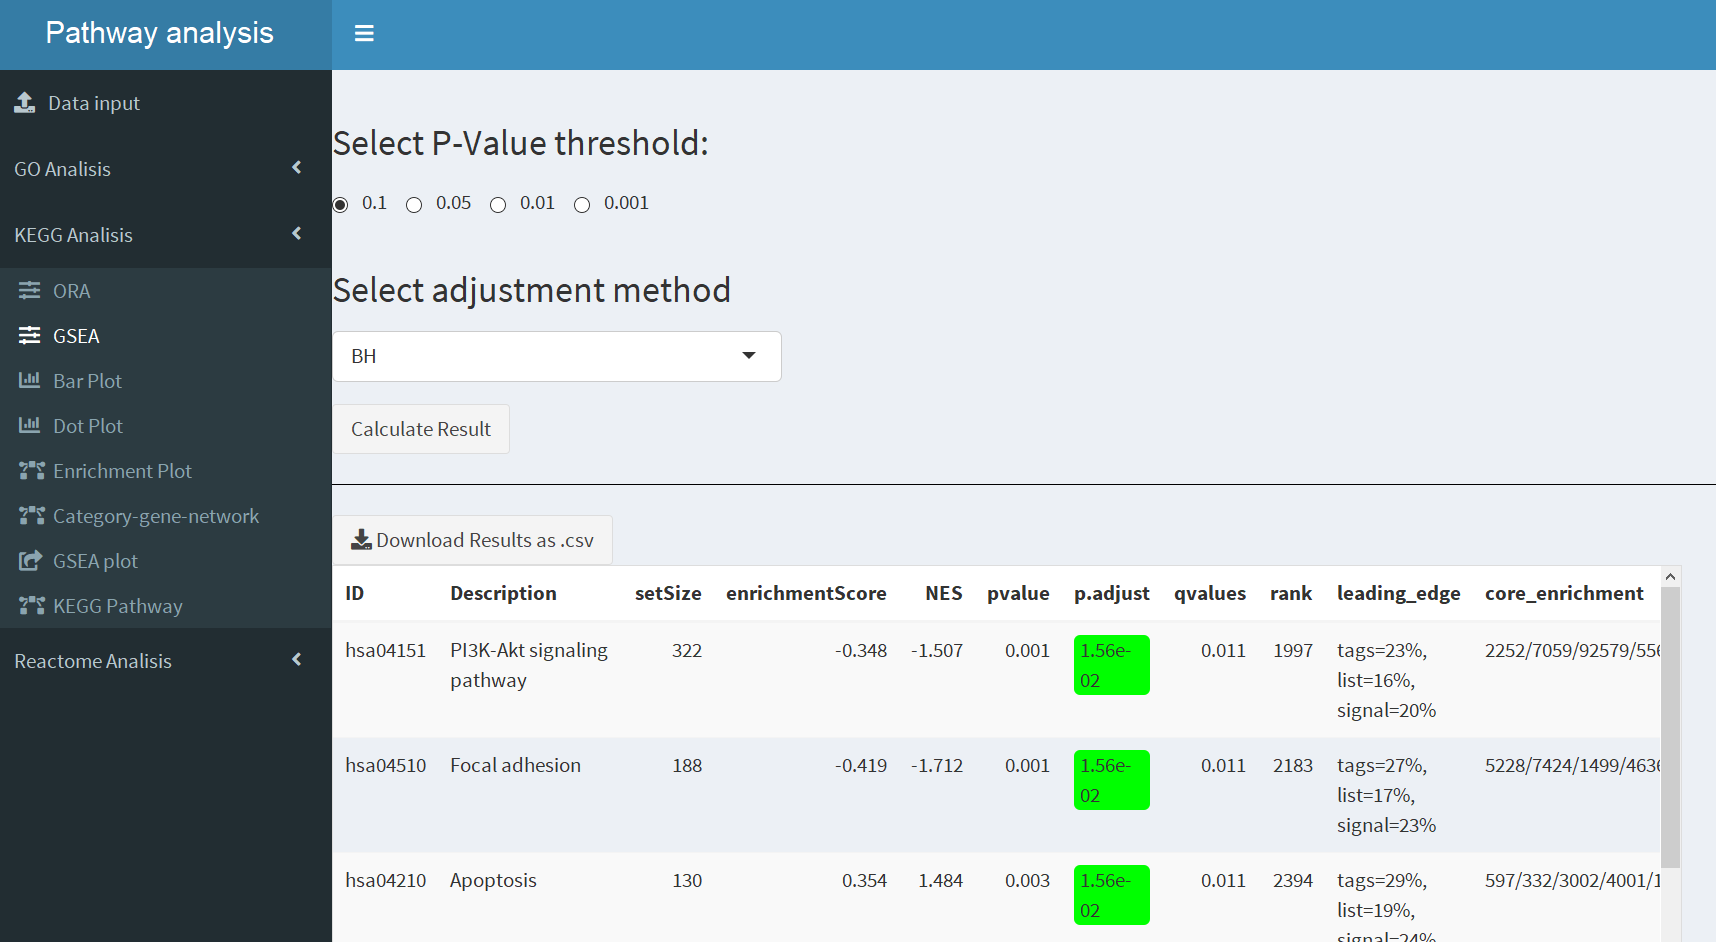
\includegraphics[width=0.9\textwidth]{App_F12_Items_KEGG_GSEA.png} 
\caption{El resultat de l'anàlisi GSEA. KEGG.}
\end{figure}

\subsubsection{Reactome}
Per completar l'anàlisi l'usuari pot calcular GSEA per a base de dades Reactome. Com als altres casos utilitzo el paquet \helvetica{clusterProfiler} i específicament la funció \helvetica{gsePathway()}

\begin{figure}[H]
\centering
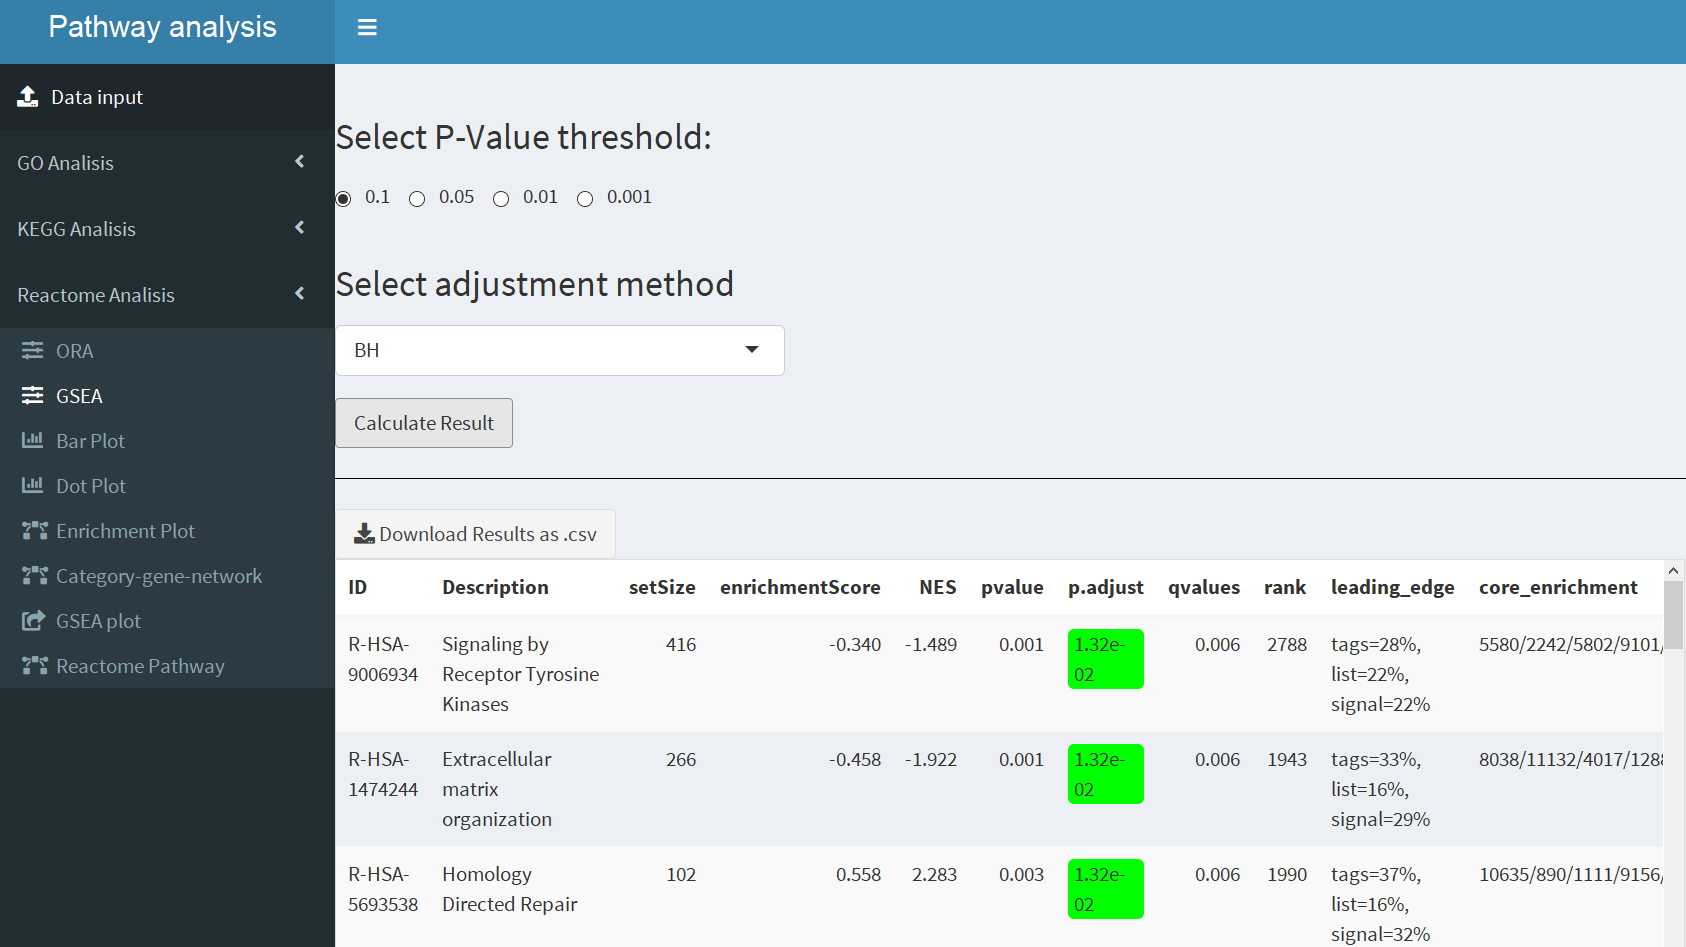
\includegraphics[width=0.9\textwidth]{App_F13_Items_RA_GSEA.png} 
\caption{El resultat d'anàlisi GSEA. Reactome.}
\end{figure}

\subsection{Bar-Plots}
Els resultats de \helvetica{enrichGO}, \helvetica{enrichKEGG} i \helvetica{enrichPathway} es poden visualitzar amb el gràfic de barres. L'usuari pot elegir el nombre de les categories visualitzades entre 2 i 30. Es dona l'opció per descarregar el gràfic en format .png.

\begin{figure}[H]
\centering
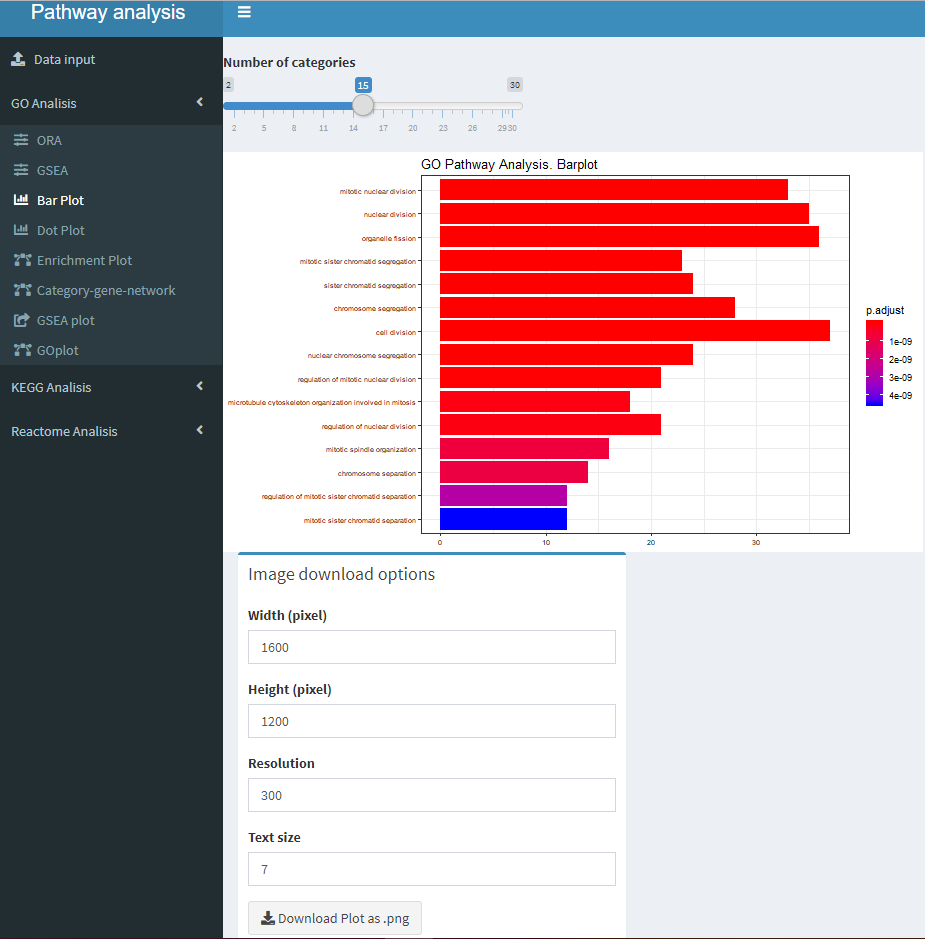
\includegraphics[width=0.9\textwidth]{App_F14_Items_GO_BarPlot.png} 
\caption{Bar-Plot. GO.}
\end{figure}

\subsection{Dot-Plots}

El \textit{dot plot} visualitza addicionalment el \textit{gen ratio}. També aquí l'usuari pot seleccionar el nombre de categories.


\begin{figure}[H]
\centering
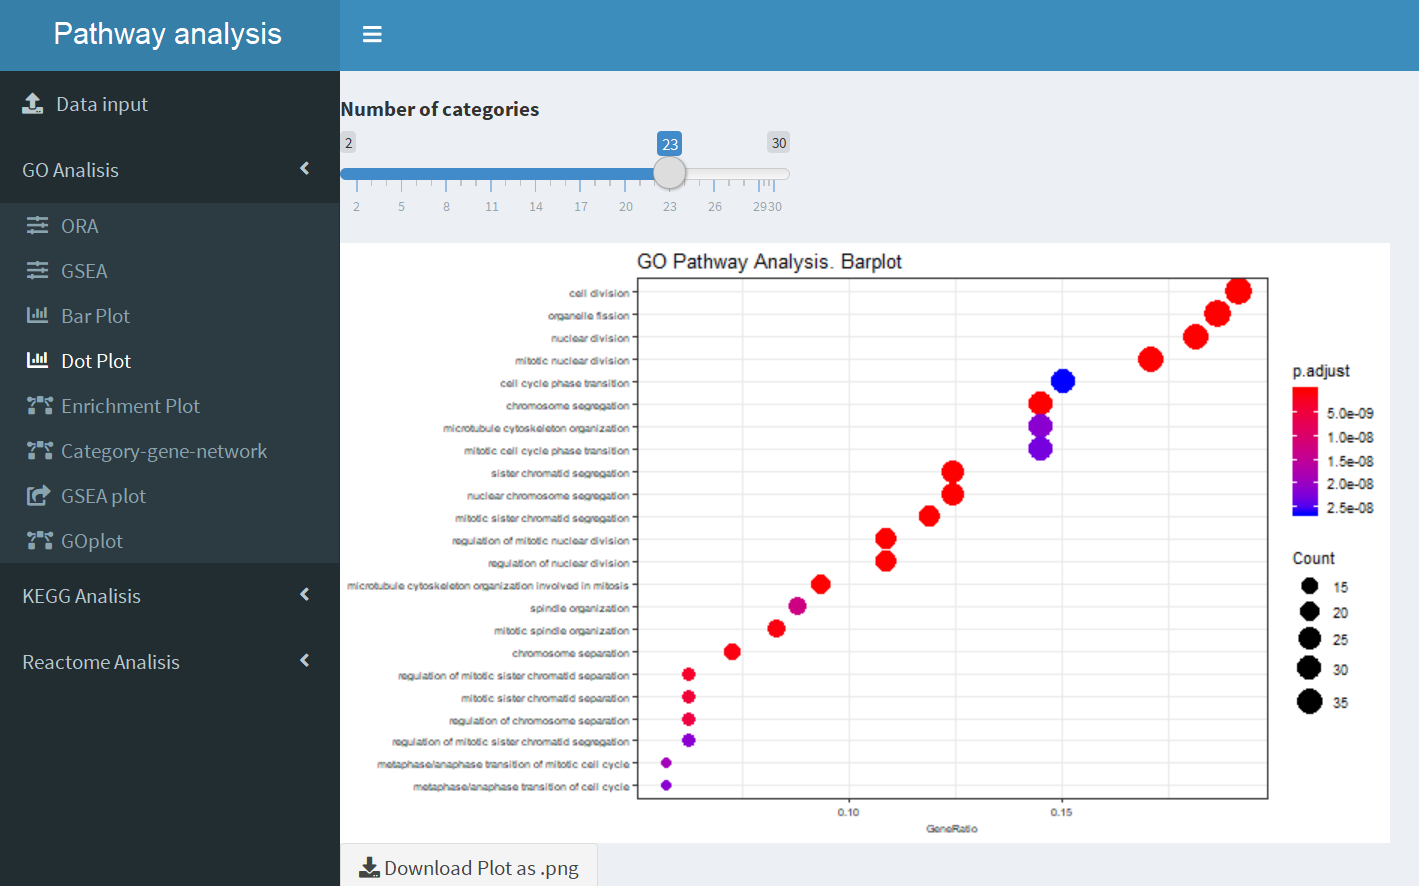
\includegraphics[width=0.9\textwidth]{App_F15_Items_GO_DotPlot.png} 
\caption{Bar-Plot. GO.}
\end{figure}

\subsection{Enrichment Plots}

\begin{figure}[H]
\centering
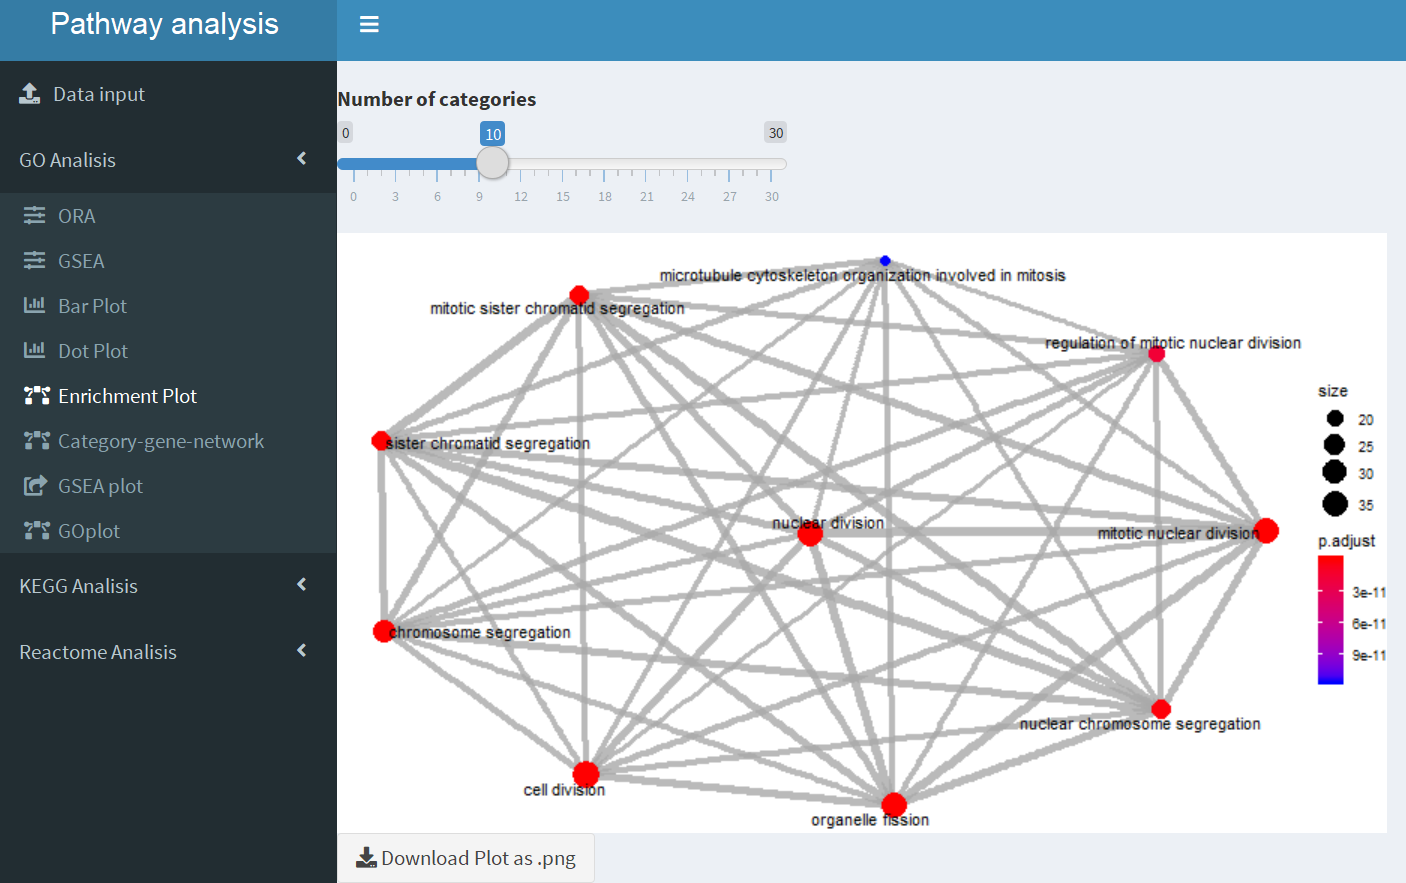
\includegraphics[width=0.9\textwidth]{App_F16_Items_GO_Emap.png} 
\caption{Bar-Plot. GO.}
\end{figure}

\subsection{Category-Gene-Network Plot}

\begin{figure}[H]
\centering
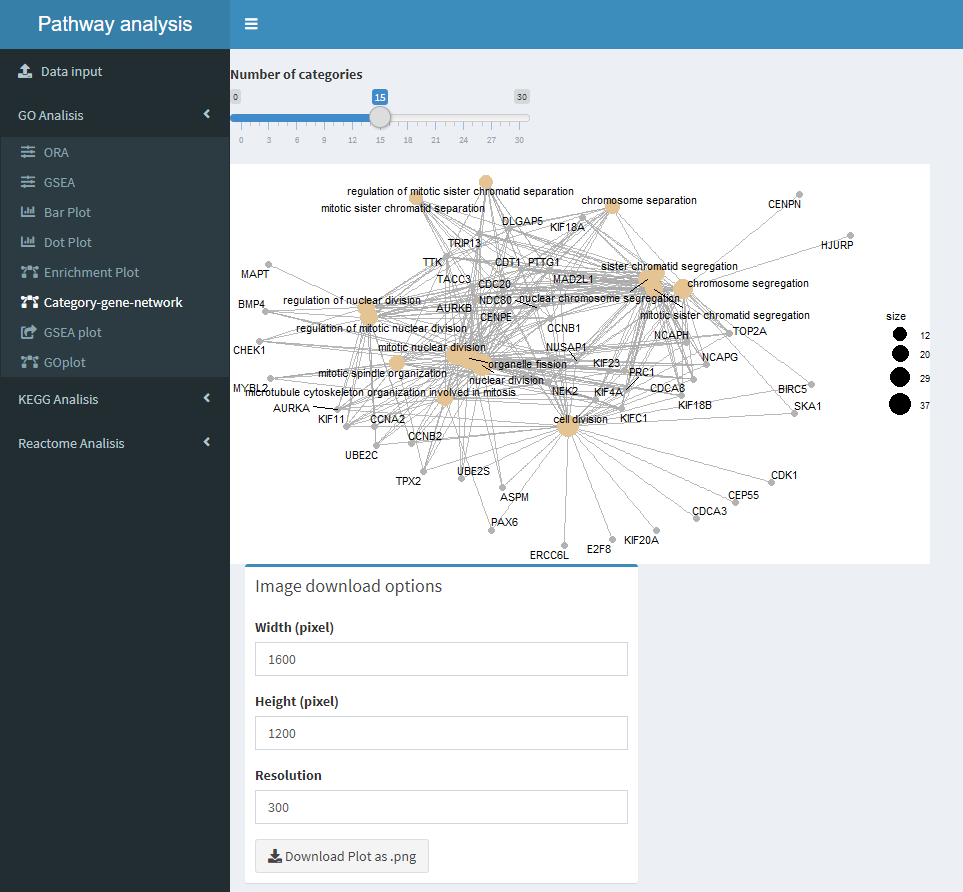
\includegraphics[width=0.9\textwidth]{App_F17_Items_GO_CnetPlot.png} 
\caption{Category-Gene-Network Plot. GO.}
\end{figure}

\subsection{GSEA Plot}
L'usuari pot visualitzar una de les categories disponibles via \textit{dropdown list}. El llistat inclou totes les rutes generades durant l'anàlisi GSEA en els apartats \textit{Go Analysis}$\rightarrow$\textit{GSEA}; \textit{KEGG}$\rightarrow$\textit{GSEA}
\begin{figure}[H]
\centering
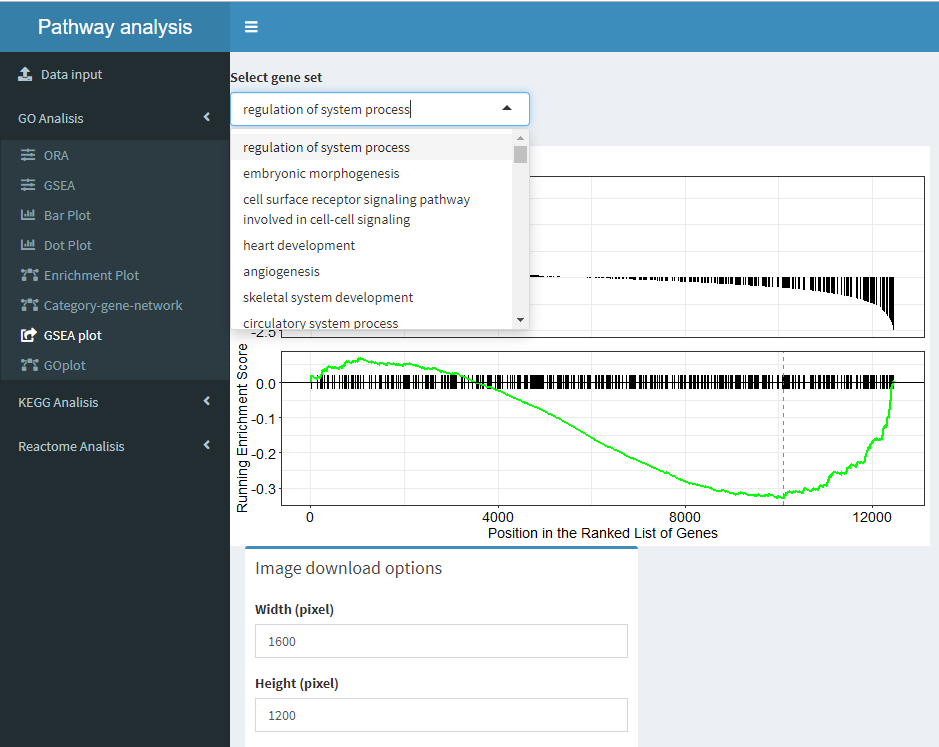
\includegraphics[width=0.9\textwidth]{App_F18_Items_GO_GSEA_Plot.png} 
\caption{GSEA Plot. GO.}
\end{figure}


\section{L'anàlisi específic de GO, KEGG i Reactome}

\subsection{GO Plot}

\begin{figure}[H]
\centering
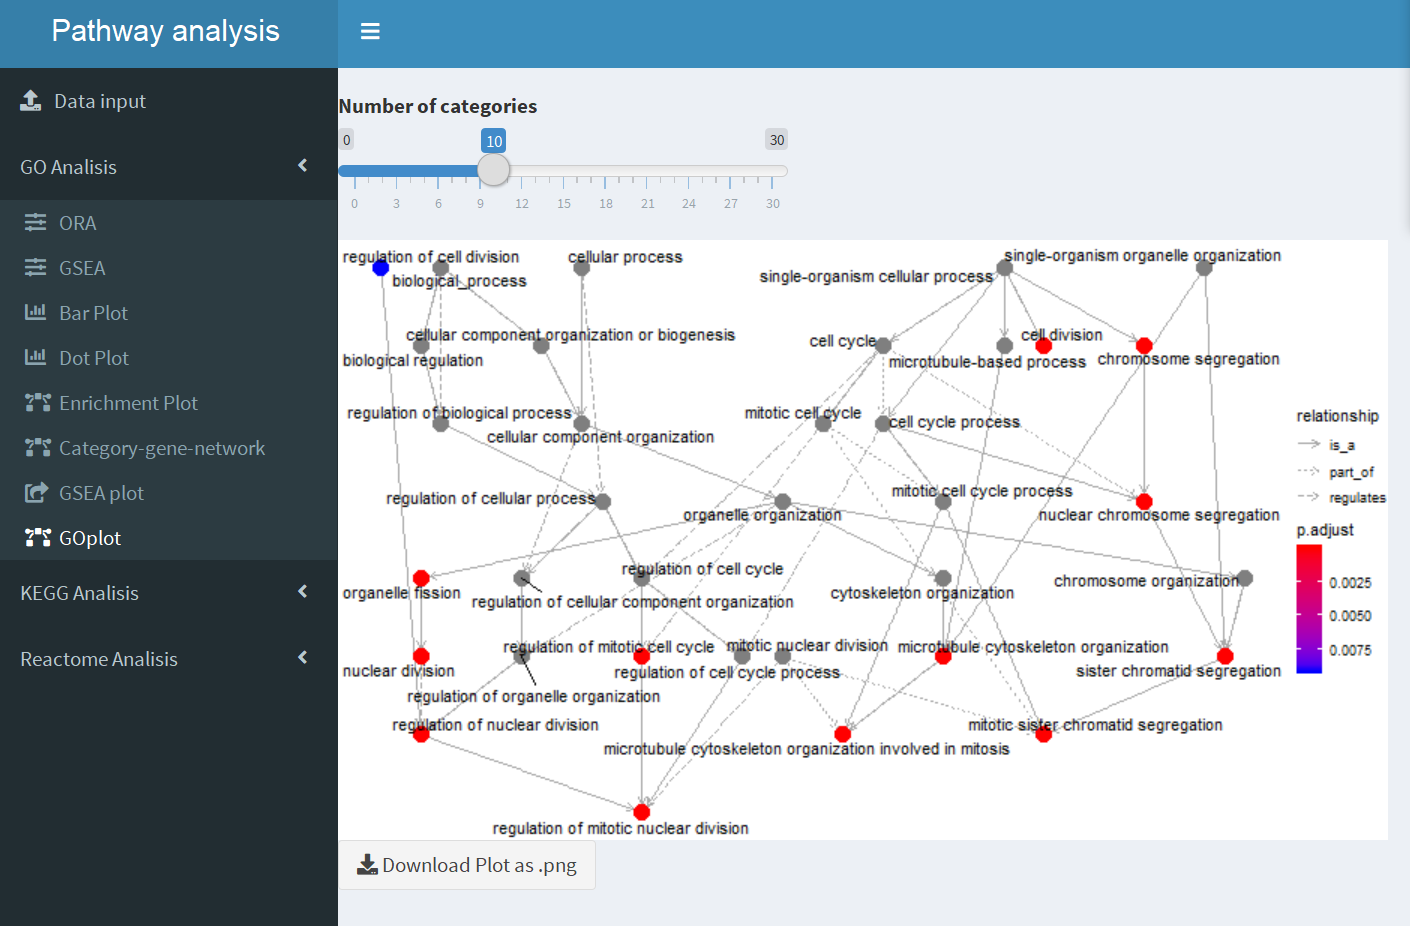
\includegraphics[width=0.9\textwidth]{App_F19_Items_GO_GOPlot.png} 
\caption{GO Plot}
\end{figure}

\subsection{KEGG Pathway}


\begin{figure}[H]
\centering
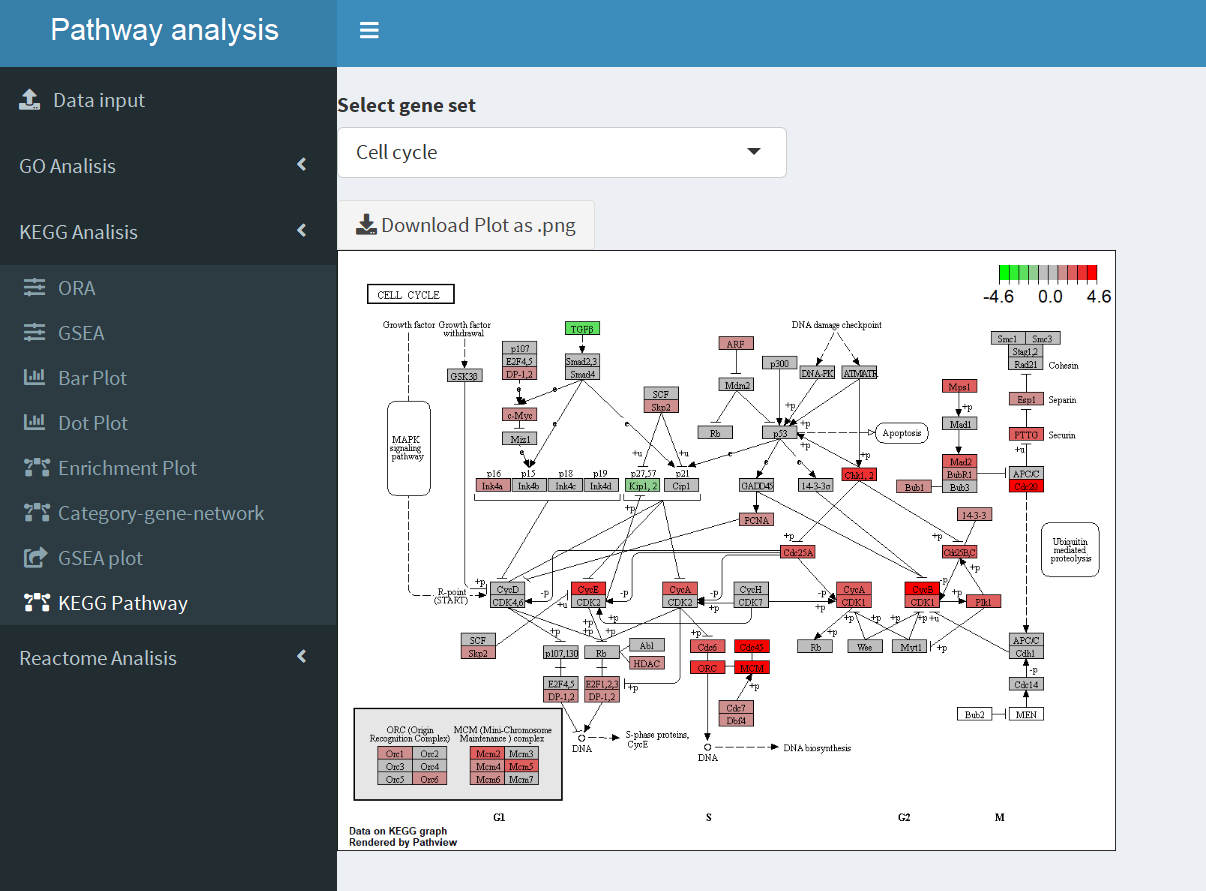
\includegraphics[width=0.9\textwidth]{App_F20_Items_KEGG_KEGGPathway.png} 
\caption{KEGG pathway}
\end{figure}

\subsection{Reactome Pathway}

\begin{figure}[H]
\centering
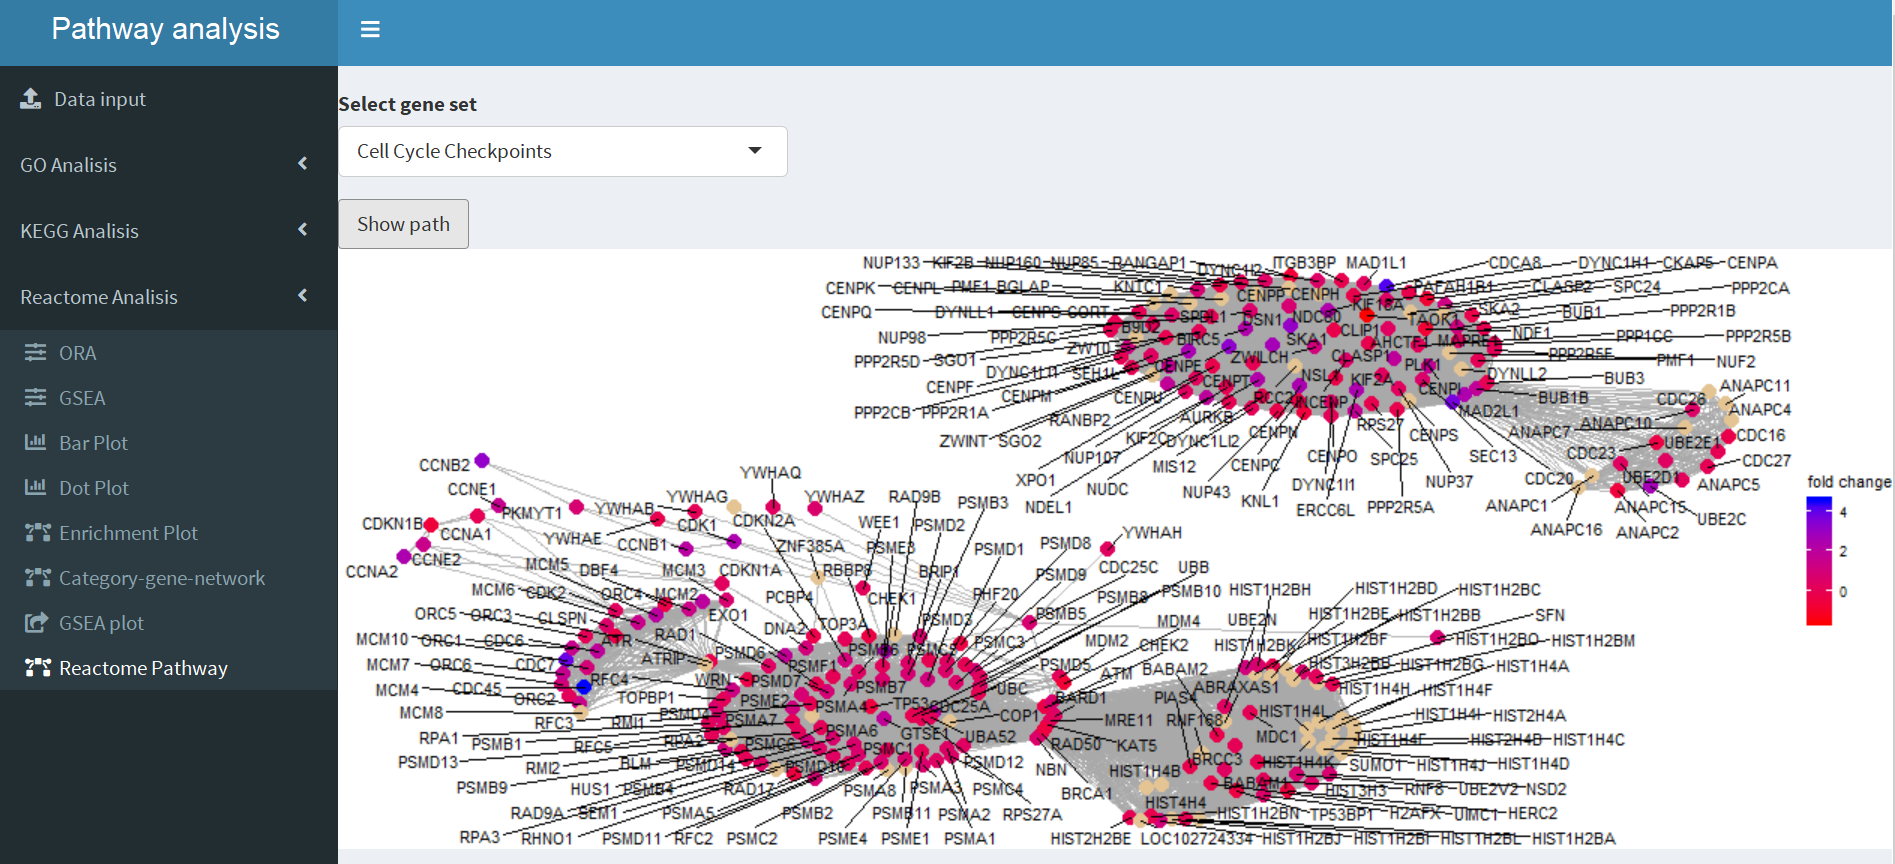
\includegraphics[width=0.9\textwidth]{App_F21_Items_RA_RAPathway.png} 
\caption{Reactome pathway}
\end{figure}



\section{Validació dels resultats}

Per validar l'aplicació he intentat trobar estudis que investiguin les espècies diferents i utilitzin com el tipo d'experiment o bé \textit{Microarrays} o bé \textit{NGS (New Generation Sequencing}. En la base de dades \href{https://www.ncbi.nlm.nih.gov/geo/}{GEO (Gene Expression Omnibus)} he elegit els estudis següents:

\begin{center}
 \begin{tabular}{||c  | c | c | c ||} 
 \hline 
 Estudi & GEO ID & Espècie & Tipo d'experiment \\ [0.5ex] 
 \hline\hline
 \cite{li2017zbtb7b}  & \href{https://www.ncbi.nlm.nih.gov/geo/query/acc.cgi?acc=GSE100924}{GSE100924}& Mus musculus  & Microarrays  \\ 
 \hline
\end{tabular}
\end{center}

L'aplicació necessita un arxiu amb les IDs de Entrez i els LogChanges. Malauradament GEO no disposa d'aquestes dades. Només té les dades en format .cel. Per tant, primer s'hauria fer els pasos d'anàlisi de dades d'expressió per derivar les dades que m'interessen. Aquests passos inclouen: normalització d'una banda i calculació del model per derivar els LogChanges d'altra banda.   

Treballant en el projecte he notat la necessitat de fer tot el procès més segur. El moment clau era quan no he pogut trobar l'USB on he guardat el meu projecte. Ho tenia en USB perquè en treballava dels molts ordinadors diferents: de casa, de feina, en portàtil quan era de viatge. Per tan he decidit guardar tot el projecte en github.com. He creat un repositori al qual puc accedir des d'ordenadors diferents.

\begin{figure}[H]
\centering
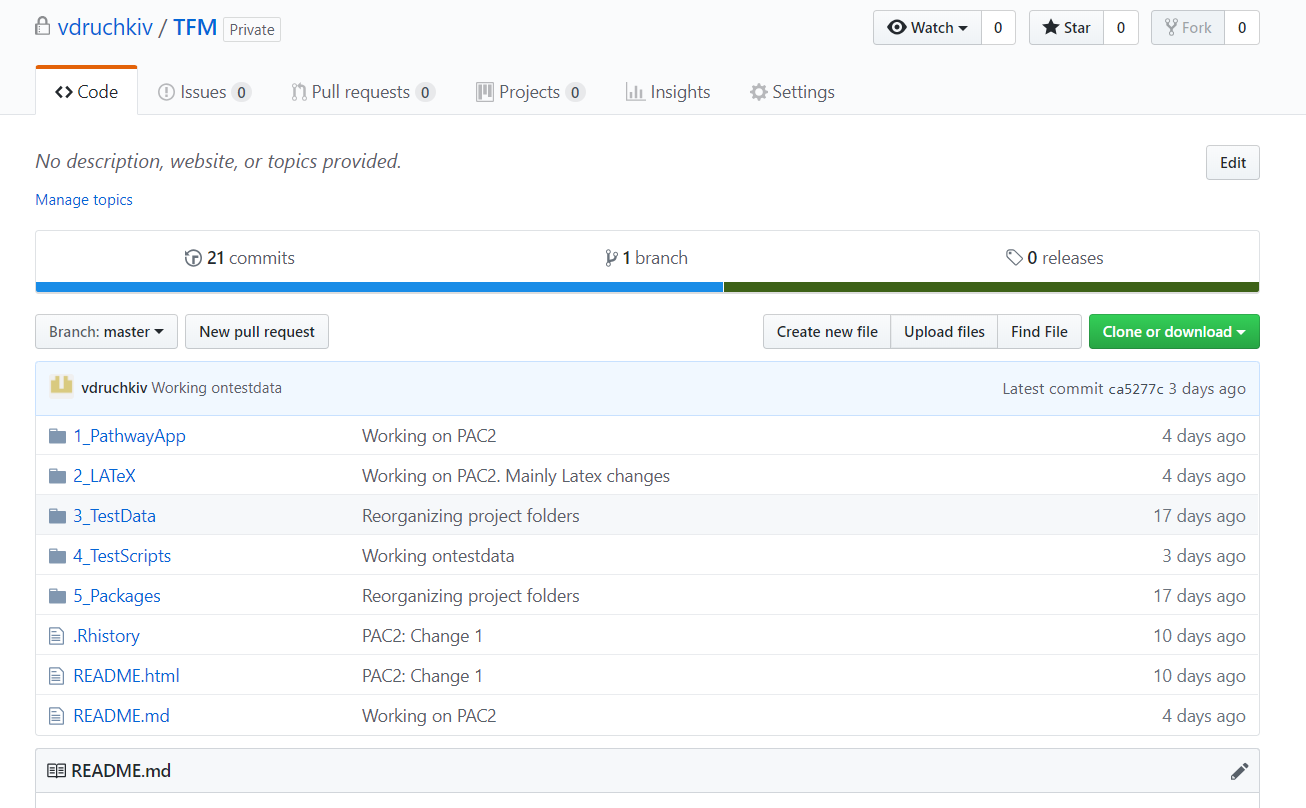
\includegraphics[width=0.9\textwidth]{GitHub.png} 
\caption{Github repositori del TFM}
\end{figure}

\bibliography{references}
\bibliographystyle{apalike}
\end{document}

